\documentclass{bioinfo}
\copyrightyear{2005}
\pubyear{2005}

\usepackage[usenames,dvipsnames]{xcolor}
\usepackage{xspace}

\newcommand{\todo}[1]{\textcolor{orange}{\textbf{TODO}: #1}} %~\\ 
\newcommand{\unsure}[1]{\textcolor{Mulberry}{\textbf{?} #1 \textbf{?}}}
\newcommand{\brainstorm}[1]{\textcolor{ProcessBlue}{\textbf{Brainstorming}: #1}}
\newcommand{\jp}[1]{\textcolor{red}{#1}}
\newcommand{\mm}[1]{\textcolor{green}{#1}}
\newcommand{\code}[1]{\texttt{#1}\xspace}
\newcommand{\rlanguage}{R\xspace}
\newcommand{\kris}[1]{\textcolor{pink}{#1}}
\def\bs{\brainstorm}
\newcommand{\wordchoice}[1]{\textcolor{red}{\textbf{#1}}}
\def\wc{\wordchoice}

\begin{document}
\firstpage{1}

\title[BioSeq in Julia]{Extending BioSeq in Julia: Contributions to an open source project}
\author[Micinski \textit{et~al}]{Kristopher Micinski\,$^{1,*}$, James Parker\,$^{2}$ and  Matthew Louis Mauriello\,$^2$\footnote{to whom correspondence should be addressed}}
\address{$^{1}$Department of Computer Science, University of Maryland, College Park}
\history{Received on XXXXX; revised on XXXXX; accepted on XXXXX}

\editor{Associate Editor: XXXXXXX}

\maketitle

\begin{abstract}

Typically, R is the programming language of choice to perform
biological computations. While the dynamic nature of the language
allows rapid programming, R suffers from poor performance and is
conducive to programming errors. One solution to this problem is the
newly developed programming language, Julia. Julia boasts many
attractive features such as a JIT compiler and a strong type system,
which address many of the shortcomings of R. Specifically, the
language produces programs with more guarantees about correctness and
runs at speeds approaching that of C. In an effort to improve
computational biology and research, we implement \unsure{parsing of
  BAM files, representation of genomic ranges, and efficient overlap
  detection} in Julia to take advantage of this new language.

\section{Motivation:}
Text Text Text  Text Text Text Text Text Text Text Text
Text  Text Text Text Text Text Text Text Text Text  Text Text Text Text Text Text Text Text Text  Text Text Text Text Text Text Text Text Text  Text Text Text Text Text Text Text Text Text  Text Text Text Text Text Text Text Text Text  Text Text Text Text Text.

\section{Results:}
Text  Text Text Text Text Text Text Text Text Text  Text Text Text Text Text Text Text Text Text  Text Text Text Text Text Text Text Text Text  Text Text Text Text Text Text

\section{Availability:}
Text  Text Text Text Text Text Text Text Text Text  Text Text Text Text Text Text Text Text Text  Text Text Text Text Text Text Text Text Text  Text

\section{Contact:} \href{name@bio.com}{name@bio.com}
\end{abstract}

\section{Introduction}

% Intro outline - problem, solution, our work/implementation

R is currently the preferred tool of the bioinformatics
community. While R works well for rapid programming, it is also
conducive to programmer error. The language is weakly typed and
coercions are implicit, which often leads to runtime errors or (worse)
code that tacitly breaks. For instance, consider the following code
that attempts to convert a data frame that is read from a file into a
matrix.

\begin{verbatim} 
raw <- read.csv(``genotypes.csv'')
genotypes <- data.matrix(raw)
\end{verbatim}

At first glance, this appears innocuous, however consider the case
when \emph{raw} contains null data (which \rlanguage represents as
\code{NA}). The \code{NA}s are implicitly coerced to \code{1} in the
matrix. If the researcher is unaware of this behavior, this coercion
can lead to incorrect analyses and results.  This is a very troubling
situation, as good scientific practice emphasizes testing and
validating \emph{all} methods for correctness.  As software is used
more and more frequently within scientific research: we need a way to
ensure the correctness of software, without adding an undue amount of
burden on the programmer.

Another issue with R is that it has poor performance. Because of
\rlanguage's highly dynamic semantics, code is executed within an
interpreter (rather than compiled, ala Fortran). Running in an
interpreter is much slower than native code executed directly by a
machine's hardware. One reason for this is that an interpreter must
read a line of code, decode it, and evaluate it. On the other hand,
native code is compiled and executed in real time by the
processor. 

Compiling \rlanguage is sometimes possible \cite{R}, but made harder
because of its dynamic type system.  The reason for this lies in the
ability of the compiler to compile an expression based on its type
(which in many languages dictates memory layout).  Consider what must
happen when the interpreter parses the expression \code{A * B}.  The
operator $\ast$ is overloaded so that it can work on a multitude of
combinations of objects (integers and vectors, matrices, etc...).  The
interpreter must first deduce the \emph{type} of the object (difficult
to do without control flow analysis \cite{cfa}), and then choose the
appropriate implementation of $\ast$ to use.  Instead, if the compiler
knows the \emph{type} of the objects, it can simply create a control
flow sequence which simply multiplies the operands, or calls a matrix
operation:

\begin{verbatim}
imul %l0 %l1
ccall multiply_matrices %p0 %p1
\end{verbatim}

% Additionally, this typing information cannot be given to the
% compiler that would generally improve performance. Instead, the
% user�fs code is interpreted by R rather than being run directly on
% the machine hardware.  This interpretation results even poorer
% performance [work in table below]. This has resulted in numerous
% alternative solutions, such as: Matlab�fs Bioinformatics Toolbox,
% BioPython, and BioLib for FORTRAN.

To address the shortcomings of \rlanguage, we investigate the new
programming language Julia and implement select functionality from
\rlanguage�fs \texttt{BioConductor} package.  Julia is a language aimed
at scientific computing and a minimal syntax, designed to be
approachable by scientists.  It actively supports users with writing
better code by providing a rich type system, native parallel
computation, simple unit testing primitives, a module system, and
other features lacking within \rlanguage. Types allow us to
syntactically specify which programs are well formed. Additionally,
performance problems commonly found in R are addressed by the Just In
Time (JIT) compiler built on top of the LLVM compiler toolkit %%\cite{}.
The JIT compiler allows the compiler to use machine specific
opportunities to highly optimize the codebase.  Because the system
uses LLVM as the underlying compiler, compilation is as efficient as
LLVM (which has a very active user community and supports efficient
compilation to many architectures).

This is apparent in Table \ref{table:languagecomparison} from
\cite{?}, which compares the performance of Julia to many different
languages. To highlight the differences in speed between R and Julia,
the table shows that Julia is 517.34 times faster than R at performing
quicksort.

A strong type system also allows the programmer to make some
guarantees about the parameters of program.  \kris{more stuff here..}

\begin{table}

\label{table:languagecomparison}
\caption{Benchmark times relative to C (smaller is better) \cite{?}.}
\end{table}

% When R is interpreting the user�fs code, each line of code is read,
% processed, and then resources are requested before the instruction
% can actually be ran. Ultimately, this means that executing the code
% will be much slower. Julia allows the user�fs code to be directly
% compiled, which allows the resulting program to be run natively. The
% processor can directly read the program binary code that corresponds
% to instructions and execute them in a much faster way.

Julia has a library for manipulating biological data called BioSeq
(Zea, 2013) , however this library does not provide the functionality
we are looking for. Currently it handles DNA sequences at the single
nucleotide level, but it does not contain data structures for looking
at regions of genes. We expand BioSeq and add additional functionality
for working with genomic range data. \unsure{ This rest of this paper
  is laid out as follows. Section 2 discusses specifically the
  functionality being added to BioSeq and discusses our hypothesis
  surrounding performance measures we anticipate being provided by
  Julia over R. Section 3 discuss the particular algorithms used in
  the countOverlaps() operation as well as discusses the SAMtools
  API. Section 4 briefly discusses the level of current
  implementation. Section 5 explores the benchmarking: procedure,
  data, results, and makes some basic conclusions. Section 6 explains
  immediate needs before public release. }

\section{System and Methods}

This project seeks to replicate a portion of BioConductor package that
is currently available in R for the Julia language. Several key
elements of this package have been selected, which includes: basic
support for \unsure{genomic data classes (i.e. IRanges, GRanges,
  etc.), support to perform union and intersection operations over
  genes, the ability to import large BAM files containing genomic
  data, and support for running overlap queries}. With respect to
loading BAM files, we have taken advantage of a Foreign Function
Interface (FFI) to take advantage of the SAMtools library.

In order to demonstrate that Julia offers performance benefits over R,
we will collect system times on the diverse set of tasks that have
been replicated in Julia.  In particular, this study will look at the
total elapse time of the countOverlaps() pipeline as well as the
elapse time of each individual set of tasks. Based on the interpreted
vs compiled nature of making code comparisons between Julia and R, we
make the following hypothesis:

H1. BAM files processing tasks and currently implement data structure
operations will show no significant differences in performance
times. The use of FFI to call SAMtools is common across both languages
and data structure operations are implemented in a naive
fashion. Therefore, it is anticipated that the Julia implementation
will be faster than R; however, this difference will not be
significant.

H2. Performing the countOverlaps() operation on the GRanges interval
object will demonstrate significant performance improvements in Julia
that result in improvement in the total elapse time of the
pipeline. The countOverlaps() operation has been implemented and
optimized for running in Julia and is expected to demonstrate
performance improvements over R implementation of the same operation.

The purpose of this study is to demonstrate the performance benefits
over R that are offered by Julia. These demonstrated benefits will
provide support for the continued deve lopment of the bioinformatics
package �gBioSeq�h.

\section{Algorithms}

\begin{figure}
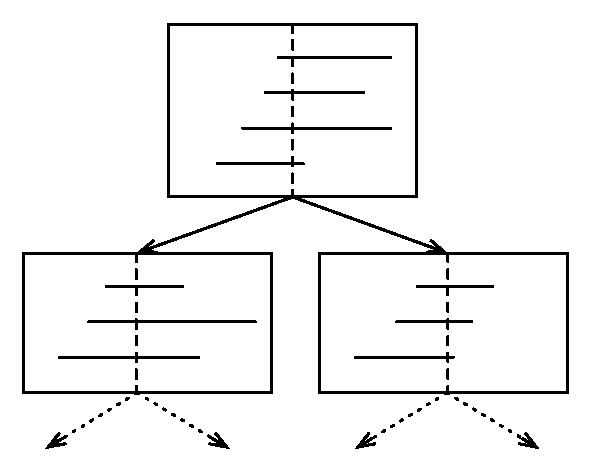
\includegraphics[width=0.5\textwidth]{images/intervaltree.pdf}
\caption{An interval tree where the intervals in each node are shown
  as sorted by the start endpoint. The dashed vertical line indicates
  the center point of the node.}
\label{fig:intervaltree}
\end{figure}

There are no novel algorithms in our implementation, however we do use
specific data structures and algorithms to make certain operations
efficient. The main example of this is the use of an interval tree. An
interval tree can be constructed out of an array of genomic
ranges. Then this data structure can be used to efficiently perform
queries to find which intervals overlap.

Interval trees are binary trees that contain intervals
\cite{deBerg:1997:CGA:261226}. Each node of the tree contains a center
point, an array of intervals that overlap the center point sorted by
the start endpoint, and another array of the same intervals sorted by
the finish endpoint. The node also stores a pointer to a left node
which is a parent of all intervals that are left of the center
point. The same is true for a right node and intervals to the right of
the center point. A diagram illustrating interval trees can be seen in
Figure \ref{fig:intervaltree} where the shown intervals are sorted by
the start endpoint.

Intervals trees can be constructed by taking the mean of the given intervals as the center point. Then intervals that overlap the center point are stored in the current node. Intervals to the left or right of the center point are then recursively split off to construct the left and right nodes until no intervals remain. This how process of construction takes $O(n \log n)$ time.

Interval trees are used to find the intervals that overlap a query
interval. This is accomplished by checking if the query interval
overlaps with a node�fs center point. If this is true then all the
intervals in that node are found to overlap. If the query interval is
left of the center point, the node�fs forward sorted array of interval
is checked if they overlap with the query. Once one of the intervals
is found to not overlap the query, the algorithm stops checking more
intervals because the intervals are sorted. The same approach is
applied to the case when the query interval is right of the center
point. After a node is finished, it recursively runs the query against
its left or right child nodes as necessary. Performing queries on
interval trees takes $O(\log n)$ time as long as the tree is
sufficiently balanced.

\section{Implementation}

We implement our codebase to mirror the implementation of the relevant
aspects of the \texttt{BioConductor} package.  When appropriate, our
types (classes in R) share the same names and functions, and our
implementation uses similar data strctures.

\subsection{\code{IRanges}}

\subsection{\code{GRanges}}

\subsection{Parsing BAM Files}

The SAM and BAM file formats represent alignments from RNA-seq data in
a standard way. \cite{samformat} A BAM file lists a large set
(hundreds of megabytes or more) of alignments given as a set of read
data and metadata (read position, forward or backward, a string
indicating status for each position, etc...).  We have implemented
machinery which allows reading of BAM files within Julia.  

Our implementation relies on the SAMtools library \cite{}: written in
C.  Julia allows interfacing with C using a simple FFI (foreign
function interface) \cite{}.  Procedures from C can be called, and the
data can be manipulated (although not all values in C can be
represented, many map onto Julia types, which are represented via
LLVM).  The \code{ccall} function allows calling C functions by
specifying their argument types and arguments (as Julia values).  The
code is then properly wrapped according to the platform's ABI and the
results are transferred back to Julia.

Representing values from C within Julia is possible when the values in
C map to a Julia type.  Julia includes various types for holding C
values, including the native C types such as \code{Uint8}, but also
pointer types such as \code{Ptr\{Void\}}.  The Julia FFI is still
evolving but looks to become a simple way to integrate scientific
libraries (written in C) to be called from Julia code.  Throughout the
development of the BAM parsing library, an author found a bug in Julia
which caused a pointer (returned from a C function) to be mishandled
by Julia's garbage collector: the bug was reported and will be fixed.

The SAMtools library allows reading extremely large alignment files
and holding the results in memory.  Because the alignment data could
be quite large, it is generally a bad idea to hold all alignments in
memory at any one time.  Instead, the file supports callback based
querying: a user queries alignments from the place in the genome in
which they are interested, and the library returns the reads.  The
reads are returned using a callback function, which is called every
time new overlapping reads (from within the region) are found.  

Our implementation harnesses the power of SAMtools, but also uses a
helper C library to create a simple wrapper which can be called from
Julia.  The reason for this library is that not all C types in
SAMtools can be easily represented in Julia: the library provides
stubs which perform operations and map them back to simple Julia
types.

Julia FFI also places the requirement that the library be dynamically
loaded (rather than statically linked).  This requires that the
SAMtools library be compiled in a position independent way: to do so
we modified the \code{Makefile} of the SAMtools library to compile a
position independent dynamic library (along with our helper stubs) to
call the code from Julia.

\section{Discussion}

\jp{these sections/subsections seem a bit weird to me} \mm{Feel free
  to change them... the format is loosely based on the guide; hector
  suggested doing our best with it, but modify as necessary} 

\subsection{Data}

Our data was collected using the system timing routines provided by
the standard libraries of Julia and R. Table X shows the average time
it takes to read in a test data file and map it to memory, run several
GRange functions, and complete multiple queries to countOverlaps()
routine.

5.2Results

With respect to H1 we found...

With respect to H2 we found...

\subsection{Limitations}

This implementation developed for this study is very preliminary. The
pipeline necessary for performing the countOverlaps() operation has
been implemented, but rigorous testing is still required to verify the
apparent deterministic behaviour beyond the limited testing that has
been performed. Additionally, the data that was used to test has been
both randomly generated or provided as sample data for a previous
project. The purpose of using randomly generated data was to verify
the correctness of the data using simple examples and then testing the
performance on various sized data sets. Using past data was done to
verify correctness of the FFI interface and SAMtools. Correctness and
performance is yet to be verified on large �greal datasets. Finally,
considerable time was invested into all three components that were
constructed for the countOverlaps() pipeline; however, most are not
optimized in the same way that countOverlaps() was and therefore are
sources of potential performance bottlenecks for future users.

\subsection{Conclusions}

R might not be the best tool for Bioinformatics. Extending the BioSeq
package for Julia will allow researchers to utilize an environment
that supports the reduction of programming errors through a typing
hierarchy, which provides improved performance over R when combined
with the JIT compiler provided by Julia. By implementing a portion of
BioSeq, we hope to encourage more development of this package by the
Bioinformatics community.

\todo{We propose that the bioinformatics community take advantage of,
  and begin developing packages for, the Julia Language
  (http://julialang.org). Julia provides a strong typing architecture
  that reduces some of the ambiguity in verifying the correctness of a
  program. Additionally, this information can be provided to a
  compiler to make some assurances about the code. The JIT compiler of
  Julia provides performances benefits over R; however, packages for
  this language are limited making R superior in terms of ease of use
  in - especially for the bioinformatics community. Without support
  from developers and researchers, this actively developing language
  will continue to be overlooked by researchers despite its many
  benefits.  }

6Future Work

This study has demonstrated the preliminary development of expansions
to the current BioSeq (Zea, 2013) package being developed for
Julia. This study showcases that Julia outperforms R in terms of
performance during our selected benchmarking operation. This expansion
includes the basic data structures, operations, and interfaces
associated with genomic ranges and intervals in R and
Bioconductor. However, further work on these objects needs to be
performed. Specifically, the genomic ranges are not fully implemented
as defined by the R specifications found in the genomic ranges
vignette (Carlson et al., 2013) and should be. We aim to complete the
functions that perform union and intersection operations across
genomic ranges and perhaps a few others as necessary..

We have also demonstrated that a simplified API wrapper for accessing
SAMtools, and BAM files, through an FFI can be replicated. The API is
very minimal, designed produce GRanges of the data specifically to
assist in performing the countOverlaps() operation. This API should
also be further developed before release \todo{expand on
  this}. Finally, general documentation and clean up tasks still need
to be performed before a large release of the project can be
considered.


\section*{Acknowledgement}

The authors would like to thank Dr. Corrada Bravo, of University of Maryland, for his guidance and direction during the course of this project. Additional thanks to the Julia  Language and BioSeq communities for providing responsive feedback and assistance with conflict resolution in this early developing environment.

%\bibliographystyle{natbib}
%\bibliographystyle{achemnat}
%\bibliographystyle{plainnat}
%\bibliographystyle{abbrv}
%\bibliographystyle{bioinformatics}
%
%\bibliographystyle{plain}
%
%\bibliography{Document}

% http://docs.julialang.org/en/latest/manual/calling-c-and-fortran-code.html
%%
\end{document}
